\documentclass{BHCexam}
\usepackage{makecell}%表格高度设置
\begin{document}
\biaoti{万门大学}
\fubiaoti{}
\maketitle
\setcounter{tocdepth}{2}
\tableofcontents
\newpage 
\section{先修知识}
\subsection{高数微积分}
$$
\int{e^x}dx = e^x + C
$$
 特殊函数的导数
$$
\int{\frac{1}{\sqrt{(1-x^2)}}}dx = \arcsin(x) + C ...
$$
线性代数

求通解特解

\subsection{2.2 2.3 常微分方程知识解析}

常微分方程
  
分类
    
 是否线性
    $$ T(\alpha \vec{v}_1 + \beta \vec{v}_2) = \alpha T(\vec{v}_1) + \beta T({\vec{v}_2}) $$
    函数$f(x)$相关的项的次数为0或1.
    
 判断下列微分方程是否为线性.

第一个$cot(x)$可以泰勒展开,可以发现右边关于$y(x)$有无穷多项,不是.

第二个同时出现了$yy'$,不是.

第三个左边明显出现了二次方,不是.

    $$ y'(x)= \cot(y(x))
    y(x)y'(x)=1
    y'(x)^2 = xy
    $$
  
    
形如下列形式的方程才是__线性微分方程__,其中$n$是有限的.
    $$
    \sum_{i=0}^{n}a_i(x)y^{(i)}(x)= b(x)
    $$
    
$a_i(x)$可以是常数,也可以是关于$x$的函数.
      
若$b(x)=0$,上式被称为__齐次线性微分方程__.
      
若$\forall y_1(x) , y_2(x)$是齐次线性方程的解.
则构成的线性组合$\alpha y_1 + \beta y_2$也是方程的解.

1. 线性代数的表述:若$y_1,y_2$是解空间的两个向量,则$y_1,y_2$的线性组合仍为解空间中的向量.

2. 映射的表述:$T(\vec{v}_1)=0,Ax=0$把所有的求导合并为算符作用于$y$上,则所有解$y$构成映射的__核__.

$$f(x)+xf'(x) + 3f''(x)=0       $$

$$ (1+x\frac{d}{dx} + 3\frac{d^2}{dx^2})f(x) = 0$$

$0$可以看作一个向量,一个算子把向量$f(x)$映射成了向量$0$.
      
若$b(x)$不恒等于0,则为__非齐次线性微分方程__.

映射的表述:线性算符$T(\vec{v}_1)=\vec{v}_2,Ax=b$
        $$f(x)+xf'(x) + 3f''(x)=b(x)=x^2       $$
            $$ (1+x\frac{d}{dx} + 3\frac{d^2}{dx^2})f(x) = b(x)=x^2$$
        
根据分类求解常微分方程

\newpage 
\section{基本性质}
\subsection{任意角的三角函数}
\subsubsection{任意角的概念}
\begin{enumerate}[1)]
\item 以$x$轴正方向为角度的起始边,把终边按逆时针方向旋转所成的角叫做\CJKunderdot{正角};按顺时针旋转的角叫做\CJKunderdot{负角}, 没有旋转所成的角叫\CJKunderdot{零角};
\item 终边相同的角:所有与$ \alpha $终边相同的角连同$ \alpha $在内可以构建一个集合$ S=\left\{\beta \left|\beta =\alpha+k\bm{\cdot}360^{\circ}\right.,k\inZ\right\} $.
\end{enumerate}
\subsubsection{弧度制}
把长度等于半径长的弧所对的圆心角叫做$ 1 $弧度的角,用符号$ rad $表示,读作弧度.\par
一般的,正角的弧度是正数,负角的弧度是负数,零角的弧度是$ 0. $如果半径为$ r $的圆的圆心角$ \alpha $所对的弧的长为$ l $,那么角$ \alpha $的弧度数的绝对值是:\[\abs{\alpha}=\dfrac{l}{r}.\]
角度与弧度对应关系:
$$\begin{array}{ll}
360^{\circ}=2\pi\  rad,&180^{\circ}=\pi\  rad;\\
1^{\circ}=\dfrac{\pi}{180}rad&1\ rad=\dfrac{180^{\circ}}{\pi}\approx57.30^{\circ}
\end{array}$$
\[
\begin{array}{|c*{11}{|c}|}
\hline
\text{度}&0^{\circ}& 30^{\circ}& 45^{\circ}& 60^{\circ}& 90^{\circ}& 120^{\circ}& 135^{\circ}&150^{\circ}&180^{\circ}&270^{\circ}&360^{\circ}\\\hline
\text{弧度}&0&\Gape[6pt]{\dfrac{\pi}{6}}&\dfrac{\pi}{4}&\dfrac{\pi}{3}&\dfrac{\pi}{2}&\dfrac{2\pi}{3}&\dfrac{3\pi}{2}&\dfrac{5\pi}{6}&\pi&\dfrac{3\pi}{2}&2\pi\\\hline
\end{array}
\]
\subsubsection{任意角的三角函数}
$ P(x,y) $是角$ \alpha $终边上异于原点的一点,$ \abs{OP} =r=\sqrt{x^2+y^2}$,则\[\sin\alpha=\dfrac{y}{r},\cos\alpha=\dfrac{x}{r},\tan\alpha=\dfrac{y}{x}.\]
其中$ x,y $都是带符号数,所以可以根据各象限内$ x,y $的正负性得到三角函数的符号规律:一 全正,二正弦,三两切(余切高考不涉及),四余弦.\par 

\subsubsection{同角三角函数关系}
两个重要的三角函数关系式:
\ding{192} $\sin^2\alpha+\cos^2\alpha=1;$\qquad
\ding{193} $ \tan\alpha=\dfrac{\sin\alpha}{\cos\alpha}.$
\subsubsection{诱导公式}

\begin{center}
\begin{tikzpicture}
\tikzmath{
\a =sqrt(3)/2;
\b =1/2;
\c =-\b;
}
\coordinate[label=below right:\footnotesize $O$](O) at(0,0);
\draw (0,0) circle (1cm);
\draw[->,>=latex] (-1.4,0)--(1.4,0)node[below](x){$x$};
\draw[->,>=latex] (0,-1.4)--(0,1.4)node[right](y){$y$};
\coordinate[label= right:\tiny $M$] (M) at(30:1);
\draw (0,0)--(30:1.4);
\draw[densely dashed] (30:1)|-(0.5,0);
\draw[densely dashed] (30:1)-|(0,0);
\coordinate[label=below:\tiny $M'$](M1)at(\a ,0);
\draw (0.3,0) arc(0:30:0.3);
\node[right](a) at (16:0.4) {\footnotesize $ \alpha$};
\coordinate[label=left:\tiny $N$] (N) at(120:1);
\coordinate[label=below:\tiny $N'$](N1)at(\c ,0);
%\coordinate[label=left:$N''$](M2)at(0 ,\a);
\draw (0,0)--(120:1.4);
\draw[densely dashed] (120:1)|-(0,0);
\draw[densely dashed] (120:1)-|(0,0);
\draw (0.4,0) arc(0:120:0.4);
\node[above](b) at (110:0.4) {\footnotesize$ \beta$};
\draw[rotate=30] (0,0) rectangle +(0.2,0.2);
\end{tikzpicture}
\end{center}

如上图所示,当$\beta=\dfrac{\pi}{2}+\alpha\text{时}, \triangle OMM' $和$ \triangle ONN' $全等,根据三角函数定义,可以得到:\[\cos\beta=\dfrac{ON'}{ON}=-\dfrac{MM'}{OM}=-\sin\alpha\]
即:\[\cos\left(\dfrac{\pi}{2}+\alpha\right)=-\sin\alpha \]
以此类推,可得:
$$ \sin\left(\dfrac{k\pi}{2}\pm\alpha\right)=\Bigg\{\begin{aligned}
&+\textfractionsolidus - \sin\alpha&k\text{为偶数},\\
&+\textfractionsolidus - \cos\alpha&k\text{为奇数}.
\end{aligned}~{(\kaishu \text{奇变偶不变,符号看象限})} $$
{\kaishu 此公式为自创精简写法,分析如下:当$ k $为奇数时,正(余)弦仍对应正(余)弦,当$ k $为偶数时,正(余)弦对应余(正)弦,右侧的正负号根据$ \dfrac{k\pi}{2}\pm\alpha $所在象限的正(余)弦值决定.}

\subsection{函数图象}
\subsubsection{正弦函数图象}
\begin{center}
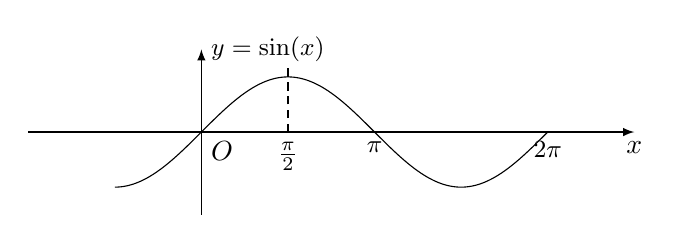
\begin{tikzpicture}[scale=0.7]
\coordinate[label=below right:$O$] (O) at(0,0);
\coordinate[label=below :\small$\pi$] (t1) at(pi,0);
\coordinate[label=below :\small$2\pi$] (t2) at(2*pi,0);
\draw[->,>=latex](-pi,0)--(2.5*pi,0)node[below](x) {$x$};
\draw[->,>=latex](0,-1.5)--(0,1.5)node[right](y) {\small $y=\sin(x)$};
\draw [domain=-pi/2:2*pi,samples=1000] plot(\x,{sin(\x r)});
\draw[densely dashed](pi/2,0)node[below](pi){$\frac{\pi}{2}$}--++(0,1.2);
\end{tikzpicture}
\end{center}
\begin{enumerate}[(1)]
\item 定义域:$x\inR$;\quad 值域:$ \left[-1,1\right] $ ;\quad 奇偶性:奇函数;
\item 对称轴:$ x=k\pi+\dfrac{\pi}{2}\left(k\inZ\right) $;\quad 对称中心:$\left(k\pi,0\right)\left(k\inZ\right)$;\quad 最小正周期:$ T=2\pi  $;
\item 单调区间:\begin{enumerate}[(i)]
\item 单调递增区间:$ \left[2k\pi-\dfrac{\pi}{2},2k\pi+\dfrac{\pi}{2}\right]\left(k\inZ\right) $;
\item 单调递减区间:$ \left[2k\pi+\dfrac{\pi}{2},2k\pi+\dfrac{3\pi}{2}\right] \left(k\inZ\right)$.
\end{enumerate}
\end{enumerate}
\subsubsection{余弦函数图象}
\begin{center}
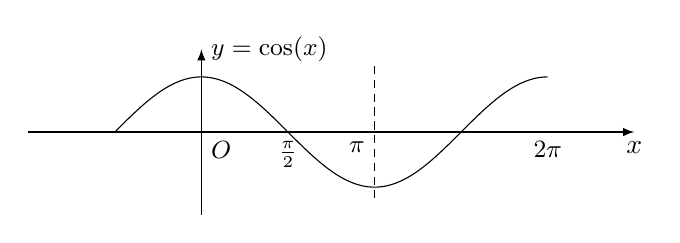
\begin{tikzpicture}[scale=0.7]
\coordinate[label=below right:\small$O$] (O) at(0,0);
\coordinate[label=below :\small $\frac{\pi}{2}$] (t1) at(pi/2,0);
\coordinate[label=below :\small $2\pi$] (t2) at(2*pi,0);
\draw[->,>=latex](-pi,0)--(2.5*pi,0)node[below](x) {$x$};
\draw[->,>=latex](0,-1.5)--(0,1.5)node[right](y) {\small $y=\cos(x)$};
\draw [domain=-pi/2:2*pi,samples=1000] plot(\x,{cos(\x r)});
\draw[densely dashed](pi,1.2)--++(0,-1.2)node[below left](pi){\small $\pi$}--++(0,-1.2);
\end{tikzpicture}
\end{center}
\begin{enumerate}[(1)]
\item 定义域:$x\inR$;\quad 值域:$ \left[-1,1\right] $;\quad 奇偶性:偶函数;
\item 对称轴:$ x=k\pi \left(k\inZ\right) $;\quad 对称中心:$\left(k\pi+\dfrac{\pi}{2},0\right)\left(k\inZ\right)$;\quad 最小正周期:$ T=2\pi  $;
\item 单调区间:\begin{enumerate}[(i)]
\item 单调递增区间:$ \left[2k\pi-\pi,2k\pi\right] \left(k\inZ\right)$;
\item 单调递减区间:$ \left[2k\pi,2k\pi+\pi\right]\left(k\inZ\right) $.
\end{enumerate}
\end{enumerate}
\subsubsection{正切函数图象}
\begin{center}
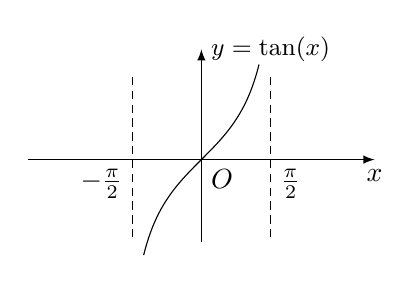
\begin{tikzpicture}[scale=0.7]
\coordinate[label=below right:$O$] (O) at(0,0);
%\coordinate[label=below :$\dfrac{\pi}{2}$] (t1) at(pi/2,0);
%\coordinate[label=below :$2\pi$] (t2) at(2*pi,0);
\draw[->,>=latex](-pi,0)--(pi,0)node[below](x) {$x$};
\draw[->,>=latex](0,-1.5)--(0,2)node[right](y) {\small $y=\tan(x)$};
\draw [domain=-pi/3:1/3*pi,samples=1000] plot(\x,{tan(\x r)});
\draw[densely dashed](2*pi/5,1.5)--++(0,-1.5)node[below right](pi){$\frac{\pi}{2}$}--++(0,-1.5);
\draw[densely dashed](-2*pi/5,1.5)--++(0,-1.5)node[below left](pi){$-\frac{\pi}{2}$}--++(0,-1.5);
\end{tikzpicture}
\end{center}
\begin{enumerate}[(1)]
\item 定义域:$\left\{x\left|x\ne k\pi+\dfrac{\pi}{2}\right.\right\}\left(k\inZ\right)$;\quad 值域:$ \mathbf{R} $;\quad 奇偶性:奇函数;
\item 对称中心:$\left(k\pi,0\right)\left(k\inZ\right)$;\quad 最小正周期:$ T=\pi  $;
\item 单调区间:单调递增区间:$ \left(k\pi-\dfrac{\pi}{2},k\pi+\dfrac{\pi}{2}\right) \left(k\inZ\right)$;
\end{enumerate}
\subsection{$y=A\sin\left(\omega x+\varphi\right)$}
\subsubsection*{$y=A\sin\left(\omega x+\varphi\right)$图象}
\begin{enumerate}[1)]
\item 用“五点法”作图:设$ z=\omega x+\varphi $,由$ z $取$ 0,\dfrac{\pi}{2},\pi,\dfrac{3\pi}{2},2\pi $来求出相应的$ x $,通过描点连线的方法画出图象.\par
{\kaishu {\heiti (注:}此处使用的$ z=\omega x+\varphi $的方法同样可以应用于求单调区间、最值等问题)}
\item 由函数$y=\sin(x)$的图象经过变换得到$y=A\sin\left(\omega x+\varphi\right)$的图象,有两种主要的途径:“先平移后伸缩”和“先伸缩后平移”
\begin{enumerate}[i)]
\item 先平移后伸缩\begin{equation*}
\begin{aligned}
y=\sin x&\xrightarrow[\text{平移}\abs{\varphi}\text{个单位}]{\text{向左}(\varphi>0)\text{或向右}(\varphi<0)}y=\sin\left(x+\varphi\right)\\
&\xrightarrow[\text{纵坐标不变}]{\text{横坐标变为原来的}\tfrac{1}{\omega}}y=\sin\left(\omega x+\varphi\right)\\
&\xrightarrow[\text{横坐标不变}]{\text{纵坐标变为原来的}A\text{倍}}y=A\sin\left(\omega x+\varphi\right)
\end{aligned}
\end{equation*}
\item 先伸缩后平移
\begin{equation*}
\begin{aligned}
y=\sin x&\xrightarrow[\text{纵坐标不变}]{\text{横坐标变为原来的}\tfrac{1}{\omega}}y=\sin\omega x\\
&\xrightarrow[\text{平移}\abs{\tfrac{\varphi}{\omega}}\text{个单位}]{\text{向左}(\varphi>0)\text{或向右}(\varphi<0)}y=\sin\left(\omega x+\varphi\right)\\&\xrightarrow[\text{横坐标不变}]{\text{纵坐标变为原来的}A\text{倍}}y=A\sin\left(\omega x+\varphi\right)
\end{aligned}
\end{equation*}
\end{enumerate}
\item 由图象求函数$y=A\sin\left(\omega x+\varphi\right)$的解析式一般步骤:
\begin{enumerate}[i)]
\item 由函数的最值确定$ A $的取值;
\item 由函数的周期确定$ \omega $的值, 周期:$ T=\dfrac{2\pi}{\abs{\omega}} $;
\item 由函数图象最高点(最低点)的坐标得到关于$ \varphi $的方程,再由$ \varphi $的范围求$ \varphi $的值.
\end{enumerate}

\item 最值:当$ x $没有范围要求时,$  A $和$ -A $分别为最大值和最小值;当$ x $有范围时,切忌将范围两端分别代入得到所谓取值范围.
\end{enumerate}
\subsubsection*{$y=A\sin\left(\omega x+\varphi\right)$的单调区间问题}
\begin{enumerate}[1)]
\item 对于选择填空题,可以直接作图得到单调区间(不推荐);
\item 通用流程:\begin{enumerate}[1)]
\item 确定$ \omega $为正,若为负,则用诱导公式转化为正;
\item 确定$ A $为正,若为负,去掉负号反向取值(求$\nearrow$改成求$ \searrow $,求$ \searrow $改成求$ \nearrow $.)
\item 令$ t=\omega x+\varphi $,得到$ y=\sin t $,根据$ y=\sin t $增区间和减区间得到$ \omega x+\varphi $的范围,进而得到$ x $的取值范围.
\end{enumerate}
\end{enumerate}
\subsubsection*{$y=A\sin\left(\omega x+\varphi\right)$在给定区间最值问题}\label{123}
对于给定区间$ x\in\left[x_1,x_2\right] $,有:
\begin{enumerate}
\item 设$ t=\omega x+\varphi $;
\item 将$ x $的取值代入$ \omega x+\varphi $中计算$ t$的取值范围;
\item 根据$ y=\sin t $的图象(标准图象)得到$ y $的最值及此时$ x $的取值$ x_0 $.
\end{enumerate}
{\kaishu \textbf{注:}对于类似$ y=f\left[g\left(x\right)\right] $类型的复合函数的相关计算问题(定义域、单调区间、比较大小等),一般可以分解为 $\begin{dcases}
		y=f\left(u\right)\\
		u=g\left(x\right)
	\end{dcases} $,通过两个基本函数的性质解题.\par
例如:$ y=sin\left(2x+\dfrac{\pi}{3}\right) $可以分解为$\begin{dcases}
	y=sin\left(t\right)\\
	t=2x+\dfrac{\pi}{3}
	\end{dcases}$,根据$ y=sin\left(t\right) $单调增区间有$ t\in\left[2k\pi-\dfrac{\pi}{2},2k\pi+\dfrac{\pi}{2}\right] \left(k\inZ\right)$,代入$ t=2x+\dfrac{\pi}{3} $即可以得到$ y $关于$ x $的单调区间.

}%
\subsection{三角恒等变换}
\subsubsection{和差公式}
如下图,在半径为$ 1 $的圆内,构建向量$ \vv{OA},~\vv{OB} $.
\begin{center}
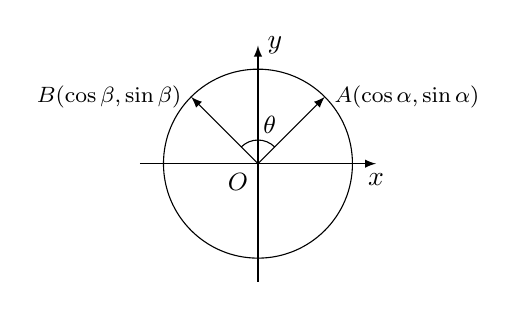
\begin{tikzpicture}
\coordinate[label=below left:\small $O$](O) at(0,0);
\draw (0,0) circle (1.2cm);
\draw[->,>=latex] (-1.5,0)--(1.5,0)node[below](x) {$x$};
\draw[->,>=latex] (0,-1.5)--(0,1.5)node[right](y) {$y$};
\draw[->,>=latex](0,0)--(45:1.2) node[right](A){\footnotesize $A(\cos\alpha,\sin\alpha)$};
\draw[->,>=latex](0,0)--(135:1.2) node[left](B){\footnotesize $B(\cos\beta,\sin\beta)$};
\draw[rotate=45] (0.3,0) arc(0:90:0.3);
\coordinate[label=\small$\theta$](t) at(60:0.3);
\end{tikzpicture}
\end{center}
根据向量夹角公式$ \cos\theta=\displaystyle\frac{\vv{OA}\bm{\cdot}\vv{OB}}{\abs{\vv{OA}}\abs{\vv{OB}}} $,将$ \vv{OA}=(\cos\alpha,\sin\alpha),\vv{OB}=(\cos\beta,\sin\beta) $代入解得:\[\cos\theta=\cos\left(\beta-\alpha\right)=\cos\alpha\cos\beta+\sin\alpha\sin\beta\]
分别令$ \alpha=-\alpha, ~\alpha=\dfrac{\pi}{2}\pm\alpha$,~由诱导公式可得:
\[\cos\left(\alpha+\beta\right)=\cos\alpha\cos\beta-\sin\alpha\sin\beta\]
\[\sin\left(\alpha+\beta\right)=\sin\alpha\cos\beta+\cos\alpha\sin\beta\]
\[\sin\left(\alpha-\beta\right)=\sin\alpha\cos\beta-\cos\alpha\sin\beta\]
在$ \sin(\alpha+\beta)\text{和} \cos(\alpha+\beta)$中令$ \beta=\alpha $得到倍角公式:

\[\begin{aligned}
\sin2\alpha=&2\sin\alpha\cos\alpha\\
\cos2\alpha=&\cos^2\alpha-\sin^2\alpha\\
=&2\cos^2\alpha-1\\
=&1-2\sin^2\alpha.
\end{aligned}\]
\subsubsection{半角公式}
\begin{enumerate}[1)]
\item $\sin ^2x=\dfrac{1-\cos2x}{2}$
\item $\cos ^2x=\dfrac{1+\cos 2x}{2}$
\end{enumerate}
\subsubsection{辅助角公式}
对于$ y=a\sin x+b\cos x $类型的三角函数的性质需要先化简为$y=A\sin\left(\omega x+\varphi\right)$形式,所以引入角$ \varphi $使其正余弦和$ a,b $对应,根据$ \sin^2\varphi+\cos^2\varphi=1 $可得到如下形式:
\begin{equation*}\begin{aligned}
a\sin x+b\cos x=&\sqrt{a^2+b^2}\left(\dfrac{a}{\sqrt{a^2+b^2}}\sin x+\dfrac{b}{\sqrt{a^2+b^2}}\cos x\right)\\
=&\sqrt{a^2+b^2}\left(\sin x\cos \varphi+\cos x\sin\varphi\right)\\
=&\sqrt{a^2+b^2}\sin\left(x+\varphi\right)~\left(\tan\varphi=\dfrac{b}{a}\right)
\end{aligned}
\end{equation*}
由此公式可看出$ \sin\varphi=\dfrac{b}{\sqrt{a^2+b^2}},~\cos\varphi=\dfrac{a}{\sqrt{a^2+b^2}} $;\\
可根据实际情况令$  \cos\varphi=\dfrac{b}{\sqrt{a^2+b^2}},~\sin\varphi=\dfrac{a}{\sqrt{a^2+b^2}} $得到辅助角公式的余弦形式.
\subsection{三角函数化简求值问题}
\subsubsection{化简“三看”原则}
\begin{enumerate}[(1)]
\item 一看“角”,~通过看角之间的差别与联系(比如出现了$ \alpha $和$ 2\alpha $就会使用倍角公式),~正确的使用公式;
\item 二看“函数名称”,~看函数名称之间的差异,从而确定使用的公式,例如:切化弦,正余弦互化;
\item 三看“结构特征”,~分析结构特征可以帮助我们找到变形的方向,常见的有“遇到分式要通分”等.
\end{enumerate}
\subsubsection{求最值问题}\begin{enumerate}[(1)]
\item $ y=a\sin x+b\cos x=\sqrt{a^2+b^2}\sin\left(\omega x+\varphi\right) $,~ 利用有界性处理(参考\ref{123});
\item $ y=a\sin^2x+b\sin x\cos x+\cos^2x \xrightarrow{\text{降次,整理}}y=A\sin 2x+B\cos2x+C=\sqrt{A^2+B^2}\sin(2x+\varphi)+C$,~其中$ \tan\varphi=\dfrac{B}{A} .$再利用有界性;
\item $ y=a\sin^2x+b\sin x+c \text{或}y=a\cos^2x+b\cos x+c(a\ne0)$,~通过$ t=\sin x $或$ t=\cos x $转化为求关于$ t $的二次函数在区间$ \left[-1,1\right]$上的最值问题;
\item $y=a\left(\sin x\pm\cos x\right)+b\sin x\bm{\cdot}\cos x $,可令$ t=\sin x\pm\cos x $,则$ \sin x\bm{\cdot}\cos x=\pm\dfrac{t^2-1}{2} $,把三角问题转化为代数问题解决;
\item $ y=\dfrac{a\sin x+c}{b\sin x+d} $或$ y=\dfrac{a\cos x+c}{b\cos x+d} $可转化为只有分母含有$ \sin x  $或$ \cos x $的函数式,还可以转化为$ \sin x=f(y) $或$ \cos x=f(y) $的形式,由正、余弦函数的有界性求解.
\item $y=\dfrac{a\sin x+c}{b\cos x+d}\left(\text{或}y=\dfrac{a\cos x+c}{b\sin x+d}\right)$,其中$ ab\ne0 $,先化为$ y=\dfrac{a}{b}\times\dfrac{\sin x+\dfrac{c}{a}}{\cos x+\dfrac{d}{b}} \text{或}y=\dfrac{a}{b}\times\dfrac{\cos x+\dfrac{c}{a}}{\sin x+\dfrac{d}{b}} $,则转化为求圆上的动点与定点连线斜率的最值问题.
\end{enumerate}
\section{解三角形}
\subsection{正弦、余弦定理}
\subsubsection{正弦定理}
在三角形$\triangle ABC$中,角$ A,B,C $所对的边为$ a,b,c $,~有$$ \dfrac{a}{\sin A}=\dfrac{b}{\sin B}=\dfrac{c}{\sin C}=2R~(R\text{\kaishu 为外接圆半径,高考没考过半径})$$
\begin{proof}
此处以直角三角形为例.如下图,设角$ A,B,C $所对的边分别为$ a,b,c $,则有:
\begin{center}
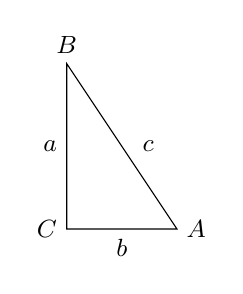
\begin{tikzpicture}[scale=0.7]
\coordinate[label=left:\small$C$](C) at(0,0);
\coordinate [label=above:\small $B$](B)at (0,3);
\coordinate [label=right:\small $A$](A)at (2,0);
\coordinate[label=right:\small$c$](c) at(1.2,1.5);
\coordinate [label=below:\small $b$](b)at (1,0);
\coordinate [label=left:\small $a$](a)at (0,1.5);
\draw(A)--(B)--(C)--cycle;
\end{tikzpicture}
\end{center}
由直角三角形对应的三角函数定义知$$  \sin A=\dfrac{a}{c},~\sin B=\dfrac{b}{c},~\sin C=\dfrac{c}{c}=1$$
即:  $$\dfrac{a}{\sin A}=\dfrac{b}{\sin B}=\dfrac{c}{\sin C}=c=2R$$
非直角三角形推导过程类似,通过构建高线得到直角三角形.
\end{proof}
正弦定理的主要作用是方程和分式中的边角互化.其原则为关于边,或是角的正弦值是否具备齐次的特征.如果齐次则可直接进行边化角或是角化边,否则不可行.
\subsubsection{余弦定理}
\begin{itemize}
\item $ c^2=a^2+b^2-2ab\cos C ~\text{或}\cos C=\dfrac{a^2+b^2-c^2}{2ab}$
\item 另外两个一样,我不想写了.
\end{itemize}
\begin{proof}
在三角形$\triangle ABC$中,角$ A,B,C $所对的边分别为$ a,b,c $,如图所示,构建向量$ \vv{a},\vv{b},\vv{c} $.
\begin{center}
\begin{tikzpicture}[scale=0.7]
\tikzmath{\c =3*sin(60);
}
\coordinate[label=left:\small$A$](A) at(0,0);
\coordinate[label=right:\small$B$](B) at(3,0);
\coordinate[label=above:\small$C$](C) at(1.5,\c);
\draw[->,>=latex](A)--(B)node[midway,below]{$\vv{c}$};
\draw[->,>=latex](C)--(A)node[midway,above left]{$\vv{b}$};
\draw[->,>=latex](C)--(B)node[midway,above right]{$\vv{a}$};
\end{tikzpicture}
\end{center}
由向量减法知:$ \vv{a}-\vv{b}=\vv{c} $两边平方得到$$ \left(\vv{a}-\vv{b}\right)^2=\vv{c}^2 $$
展开得到$$ a^2+b^2-2ab\cos C=c^2 $$\text{\kaishu(这里直接将向量模长写成边长了,代码太多了$ \ldots $)}
\end{proof}
\subsection{解三角形常用结论}
\begin{enumerate}[1)]
\item $A+B+C=\pi$;\quad $\sin\left(A+C\right)=\sin B$;\quad $\cos\left(A+C\right)=-\cos B$.
\item $S=\dfrac{1}{2}ab\sin C=\dfrac{1}{2}ac\sin B=\dfrac{1}{2}bc\sin A$;
\item $ \sin^2A+\sin^2B-\sin A\sin B=\sin^2C \Leftrightarrow a^2+b^2-ab=c^2$
\item $b\cos C+c\cos B=a\Rightarrow \sin B\cos C+\sin C\cos B=\sin A$~(恒等式)
\item $A>B>C\Leftrightarrow a>b>c\Leftrightarrow \sin A>\sin B>\sin C\Leftrightarrow \cos A<\cos B<\cos C$
\end{enumerate}

\subsection{解三角形问题主要思路}
\subsubsection{公式适用类型}
\begin{enumerate}[1)]
\item 已知两角一边,用正弦定理,有解时,只有一解;
\item 已知两边及一边对角,用正弦定理,有解的情况(设已知$ a,b $和角$ A $):\begin{enumerate}[a)]
\item $ A $为锐角,当$ a<b\sin A $时无解;若$ A $为钝角,当$ a=b,a<b $时均无解;
\item 若为求第三边问题,也可以通过余弦定理构造一元二次方程求解.
\end{enumerate}
\item 已知三边,用余弦定理,有解时,只有一解;
\item 已知两边及夹角,用余弦定理,必有一解.
\end{enumerate}
\subsubsection{解三角形最值问题}
\begin{enumerate}[(1)]
\item 利用正弦定理将边转化为角,通过三角恒等变换转化为$ y=A\sin\left(\omega x+\varphi\right) $,在满足内角和为$ \pi $的范围内求最值.
\item 对于某些乘法的最值(例如面积最大值)利用余弦定理转化为边的形式,利用基本不等式$ a^2+b^2\ge2ab $求最值.
\end{enumerate}
\include{gaokaosection}

\end{document}
